% Options for packages loaded elsewhere
\PassOptionsToPackage{unicode}{hyperref}
\PassOptionsToPackage{hyphens}{url}
\PassOptionsToPackage{dvipsnames,svgnames,x11names}{xcolor}
%
\documentclass[
  ignorenonframetext,
  aspectratio=169,
]{beamer}
\usepackage{pgfpages}
\setbeamertemplate{caption}[numbered]
\setbeamertemplate{caption label separator}{: }
\setbeamercolor{caption name}{fg=normal text.fg}
\beamertemplatenavigationsymbolshorizontal
% Prevent slide breaks in the middle of a paragraph
\widowpenalties 1 10000
\raggedbottom
\setbeamertemplate{part page}{
  \centering
  \begin{beamercolorbox}[sep=16pt,center]{part title}
    \usebeamerfont{part title}\insertpart\par
  \end{beamercolorbox}
}
\setbeamertemplate{section page}{
  \centering
  \begin{beamercolorbox}[sep=12pt,center]{part title}
    \usebeamerfont{section title}\insertsection\par
  \end{beamercolorbox}
}
\setbeamertemplate{subsection page}{
  \centering
  \begin{beamercolorbox}[sep=8pt,center]{part title}
    \usebeamerfont{subsection title}\insertsubsection\par
  \end{beamercolorbox}
}
\AtBeginPart{
  \frame{\partpage}
}
\AtBeginSection{
  \ifbibliography
  \else
    \frame{\sectionpage}
  \fi
}
\AtBeginSubsection{
  \frame{\subsectionpage}
}

\usepackage{amsmath,amssymb}
\usepackage{iftex}
\ifPDFTeX
  \usepackage[T1]{fontenc}
  \usepackage[utf8]{inputenc}
  \usepackage{textcomp} % provide euro and other symbols
\else % if luatex or xetex
  \usepackage{unicode-math}
  \defaultfontfeatures{Scale=MatchLowercase}
  \defaultfontfeatures[\rmfamily]{Ligatures=TeX,Scale=1}
\fi
\usetheme[]{Hannover}
\usecolortheme{rose}
\usepackage[]{libertinus}
\ifPDFTeX\else  
    % xetex/luatex font selection
\fi
% Use upquote if available, for straight quotes in verbatim environments
\IfFileExists{upquote.sty}{\usepackage{upquote}}{}
\IfFileExists{microtype.sty}{% use microtype if available
  \usepackage[]{microtype}
  \UseMicrotypeSet[protrusion]{basicmath} % disable protrusion for tt fonts
}{}
\makeatletter
\@ifundefined{KOMAClassName}{% if non-KOMA class
  \IfFileExists{parskip.sty}{%
    \usepackage{parskip}
  }{% else
    \setlength{\parindent}{0pt}
    \setlength{\parskip}{6pt plus 2pt minus 1pt}}
}{% if KOMA class
  \KOMAoptions{parskip=half}}
\makeatother
\usepackage{xcolor}
\newif\ifbibliography
\setlength{\emergencystretch}{3em} % prevent overfull lines
\setcounter{secnumdepth}{-\maxdimen} % remove section numbering


\providecommand{\tightlist}{%
  \setlength{\itemsep}{0pt}\setlength{\parskip}{0pt}}\usepackage{longtable,booktabs,array}
\usepackage{calc} % for calculating minipage widths
\usepackage{caption}
% Make caption package work with longtable
\makeatletter
\def\fnum@table{\tablename~\thetable}
\makeatother
\usepackage{graphicx}
\makeatletter
\def\maxwidth{\ifdim\Gin@nat@width>\linewidth\linewidth\else\Gin@nat@width\fi}
\def\maxheight{\ifdim\Gin@nat@height>\textheight\textheight\else\Gin@nat@height\fi}
\makeatother
% Scale images if necessary, so that they will not overflow the page
% margins by default, and it is still possible to overwrite the defaults
% using explicit options in \includegraphics[width, height, ...]{}
\setkeys{Gin}{width=\maxwidth,height=\maxheight,keepaspectratio}
% Set default figure placement to htbp
\makeatletter
\def\fps@figure{htbp}
\makeatother

\makeatletter
\@ifpackageloaded{caption}{}{\usepackage{caption}}
\AtBeginDocument{%
\ifdefined\contentsname
  \renewcommand*\contentsname{Table of contents}
\else
  \newcommand\contentsname{Table of contents}
\fi
\ifdefined\listfigurename
  \renewcommand*\listfigurename{List of Figures}
\else
  \newcommand\listfigurename{List of Figures}
\fi
\ifdefined\listtablename
  \renewcommand*\listtablename{List of Tables}
\else
  \newcommand\listtablename{List of Tables}
\fi
\ifdefined\figurename
  \renewcommand*\figurename{Figure}
\else
  \newcommand\figurename{Figure}
\fi
\ifdefined\tablename
  \renewcommand*\tablename{Table}
\else
  \newcommand\tablename{Table}
\fi
}
\@ifpackageloaded{float}{}{\usepackage{float}}
\floatstyle{ruled}
\@ifundefined{c@chapter}{\newfloat{codelisting}{h}{lop}}{\newfloat{codelisting}{h}{lop}[chapter]}
\floatname{codelisting}{Listing}
\newcommand*\listoflistings{\listof{codelisting}{List of Listings}}
\makeatother
\makeatletter
\makeatother
\makeatletter
\@ifpackageloaded{caption}{}{\usepackage{caption}}
\@ifpackageloaded{subcaption}{}{\usepackage{subcaption}}
\makeatother
\ifLuaTeX
  \usepackage{selnolig}  % disable illegal ligatures
\fi
\usepackage{bookmark}

\IfFileExists{xurl.sty}{\usepackage{xurl}}{} % add URL line breaks if available
\urlstyle{same} % disable monospaced font for URLs
\hypersetup{
  pdftitle={Belonging and Exclusion},
  pdfauthor={Usman Afzali, PhD - Postdoc Fellow},
  colorlinks=true,
  linkcolor={Maroon},
  filecolor={Maroon},
  citecolor={Blue},
  urlcolor={Blue},
  pdfcreator={LaTeX via pandoc}}

\title{Belonging and Exclusion}
\subtitle{The Psychology of Identity Crisis in a Diverse World}
\author{Usman Afzali, PhD - Postdoc Fellow}
\date{2024-05-31}
\institute{Uni of Canterbury}
\logo{
\includegraphics{mds.png}}

\begin{document}
\frame{\titlepage}

\begin{frame}{Institutional Partners}
\phantomsection\label{institutional-partners}
\begin{figure}

\begin{minipage}{\linewidth}
\begin{center}

\includegraphics[width=0.6\textwidth,height=\textheight]{mds.png}
\end{center}

\includegraphics{sponsors.png}\end{minipage}%

\end{figure}%
\end{frame}

\begin{frame}{Outline}
\phantomsection\label{outline}
\begin{itemize}
\tightlist
\item
  Social perspective
\item
  Developmental perspective
\item
  Identity denial
\item
  Negative consequences
\item
  What to do?
\end{itemize}
\end{frame}

\section{What is your perception from the term
``identity''?}\label{what-is-your-perception-from-the-term-identity}

\section{Social Identity}\label{social-identity}

\begin{frame}{Social Identity}
\phantomsection\label{social-identity-1}
\begin{itemize}[<+->]
\tightlist
\item
  People all over the world believe that their own nation, culture,
  language, and religion are better and more deserving than others.
\item
  But why?
\item
  Henri Tajfel (1971)
\end{itemize}
\end{frame}

\begin{frame}{Social Experiment}
\phantomsection\label{social-experiment}
\begin{columns}[c,totalwidth=8em]
\begin{column}{0.4\textwidth}
\begin{itemize}[<+->]
\tightlist
\item
  Task 1: Estimate the number of dots on each slide
\item
  Outcome: ``over-estimators'' and ``under-estimators'' Divided into two
  random groups
\item
  Task 2: allocate points to other participants that can be cashed for
  money
\end{itemize}
\end{column}

\begin{column}{0.6\textwidth}

\includegraphics{tajfel.png}
\end{column}
\end{columns}
\end{frame}

\begin{frame}[fragile]{Findings}
\phantomsection\label{findings}
\begin{itemize}[<+->]
\tightlist
\item
  More points to members of their own group than to members of the other
  group.
\item
  Ingroup favouritism (discrimination)
\item
  Replicated in many countries
\item
  \texttt{Minimal\ Groups\ Paradigm}
\end{itemize}
\end{frame}

\begin{frame}{The need for self-esteem}
\phantomsection\label{the-need-for-self-esteem}
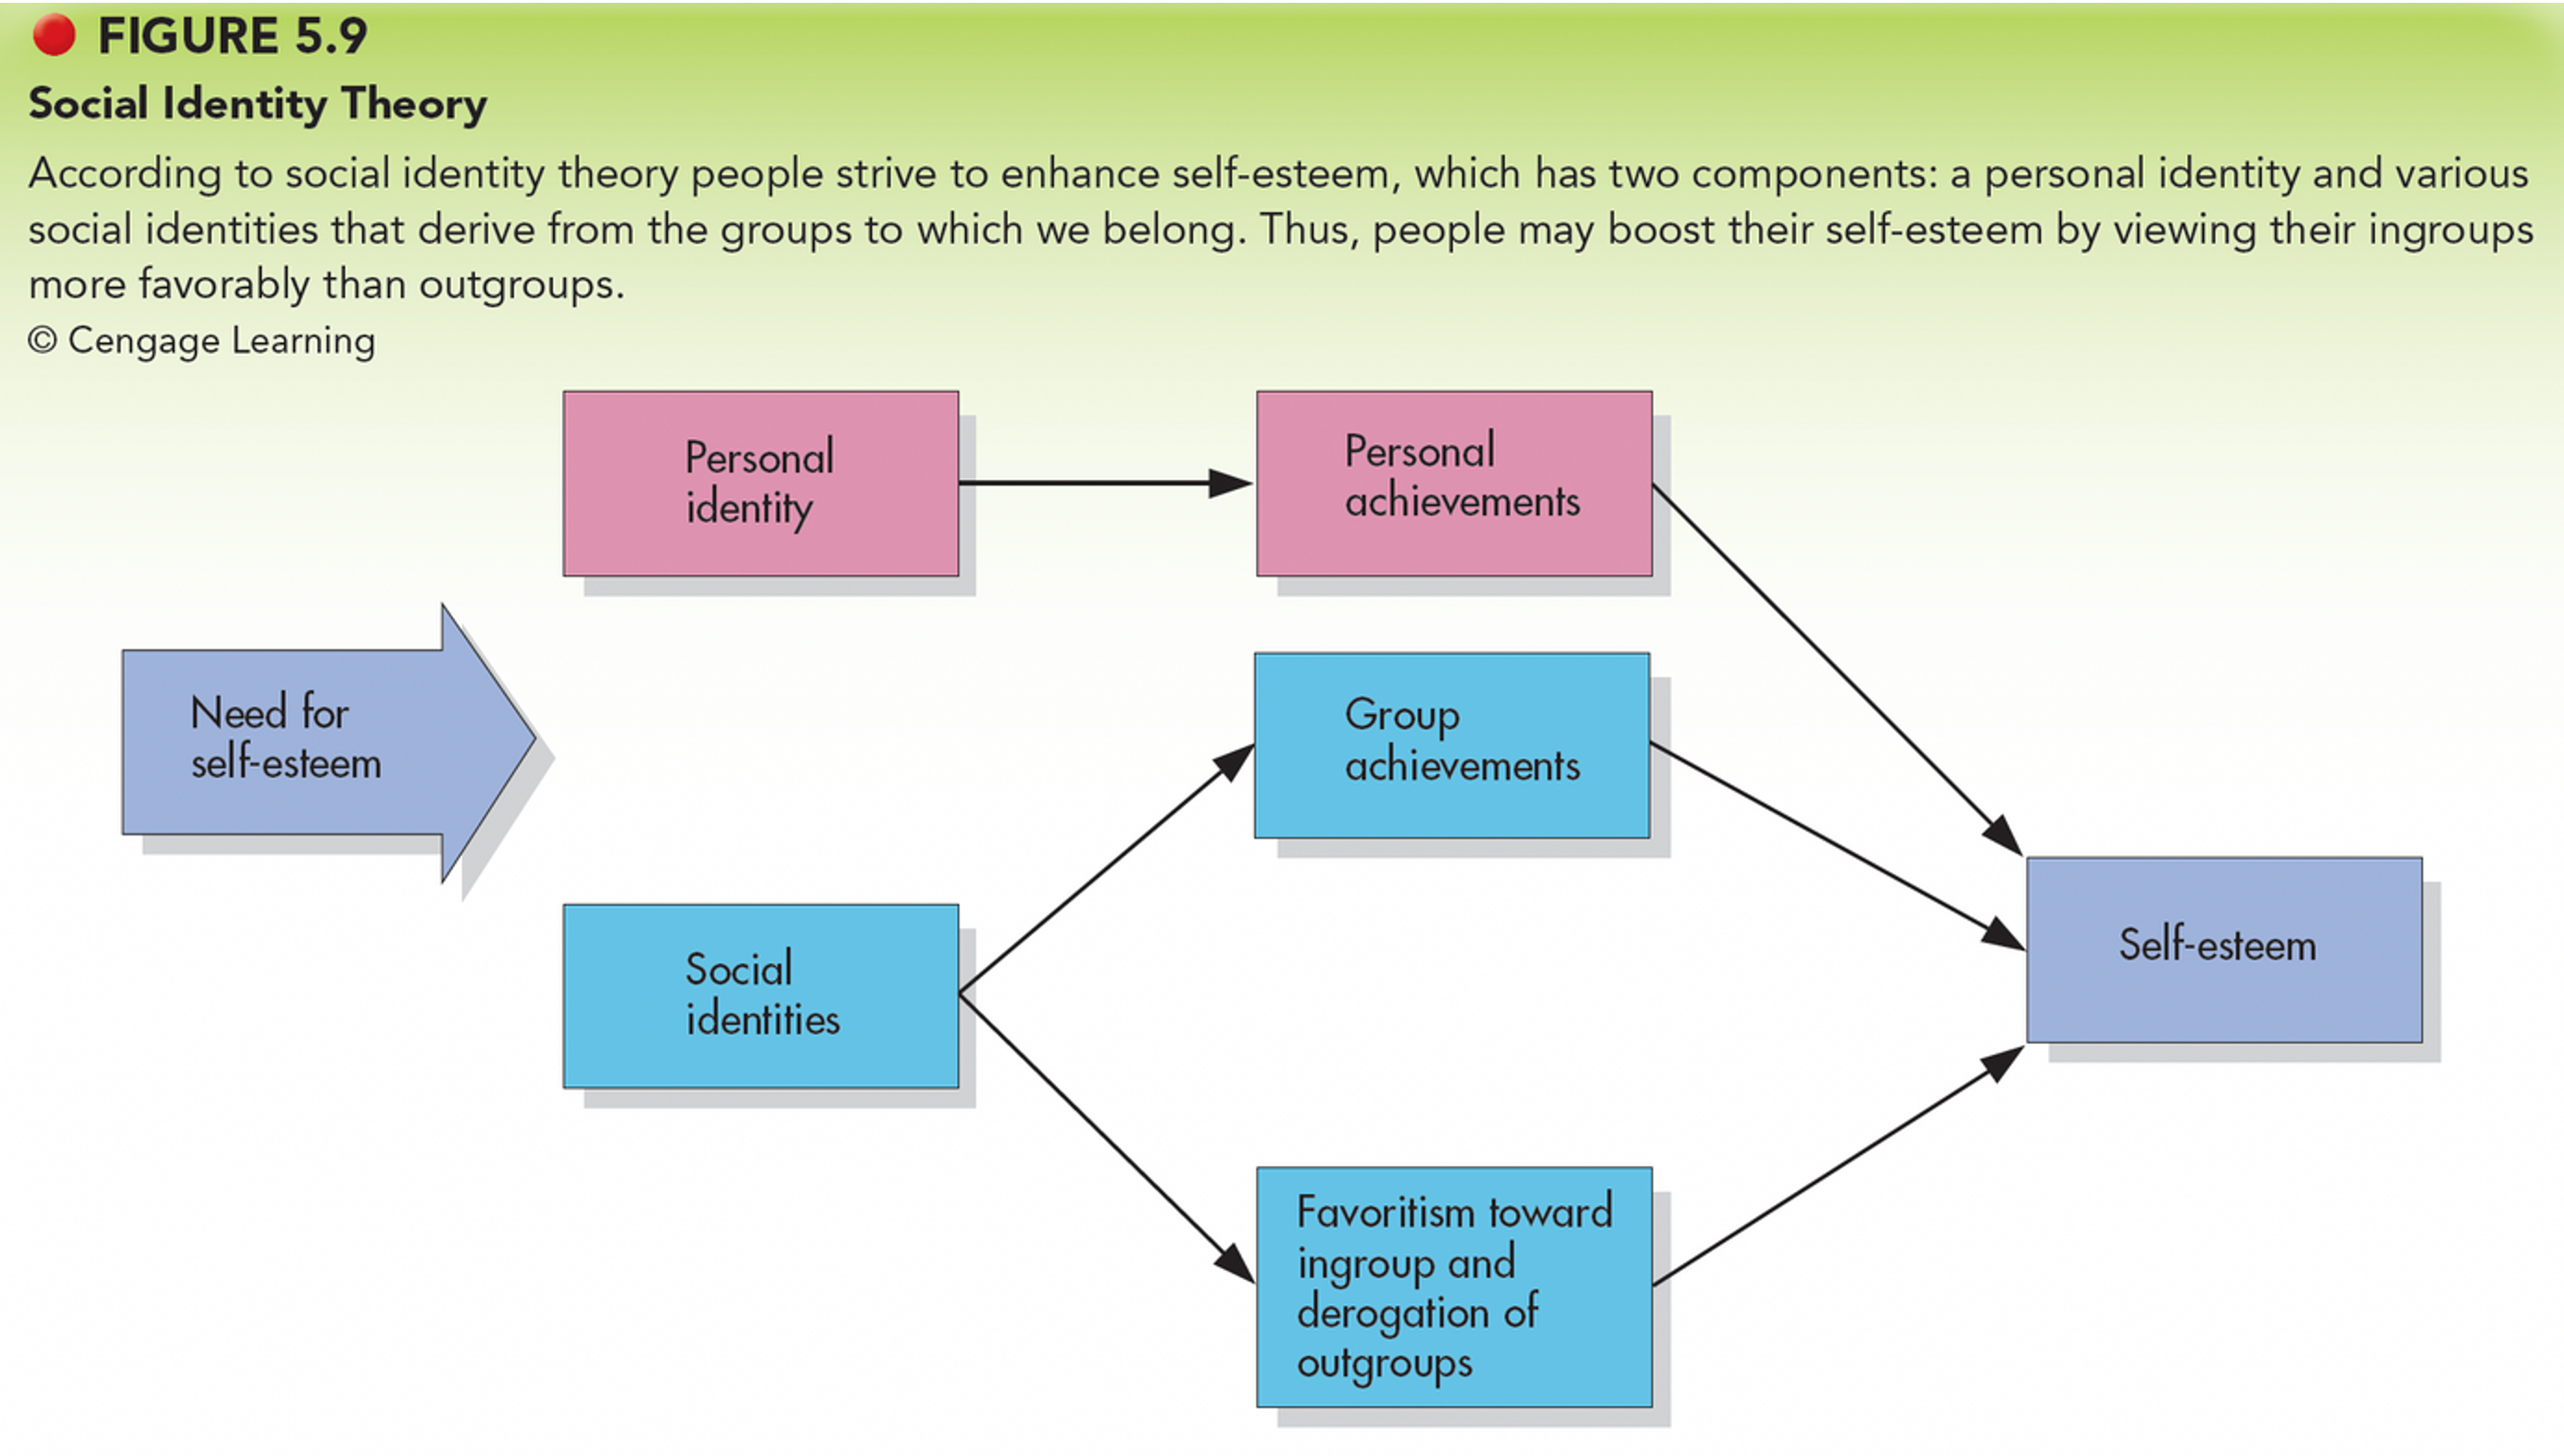
\includegraphics{selfesteem.png}
\end{frame}

\begin{frame}{Minimal Groups Paradigm}
\phantomsection\label{minimal-groups-paradigm}
\begin{itemize}[<+->]
\tightlist
\item
  Advantage: derive pride from our connections
\item
  Disadvantage: the need to belittle ``them'' in order to feel secure
  about ``us.''
\item
  Examples: Religious fervor, racial and ethnic conceit, aggressive
  nationalism, even gossiping (Bosson et al., 2006; Weaver \& Bosson,
  2011)
\item
  When people shared negative attitudes about a third party, they felt
  closer to each other.
\end{itemize}
\end{frame}

\begin{frame}{A scenario}
\phantomsection\label{a-scenario}
\begin{itemize}[<+->]
\tightlist
\item
  In New Zealand, as in many other parts of the world, Muslims often
  face stereotypes and prejudices due to their religion, culture, or
  appearance. Islamophobia, or fear and hostility toward Islam and
  Muslims, can be pervasive in society and can manifest in various
  forms, such as discrimination, harassment, or even violence.
\item
  Now, suppose an individual in New Zealand experiences a threat to
  their self-esteem, such as being criticized by colleagues at work or
  feeling excluded in a social setting. In response to this threat, they
  may seek ways to restore their sense of self-worth or superiority.
  Unfortunately, in some cases, individuals may resort to derogating
  others, including Muslims, as a means of boosting their own
  self-esteem.
\end{itemize}
\end{frame}

\begin{frame}{A scenario}
\phantomsection\label{a-scenario-1}
\begin{itemize}[<+->]
\tightlist
\item
  For example, this person might start expressing or endorsing negative
  stereotypes about Muslims, such as portraying them as terrorists,
  backward, or incompatible with Western values. By doing so, they may
  attempt to reaffirm their own identity or sense of belonging within
  the dominant culture, thus temporarily alleviating their feelings of
  insecurity or inferiority.
\item
  By linking the individual's feelings of insecurity or threat in social
  or professional settings to the broader context of Islamophobia in New
  Zealand, you can illustrate how the self-esteem maintenance model
  proposed by Fein and Spencer may play out in real-life situations,
  where individuals derogate members of stereotyped groups, such as
  Muslims, to cope with their own insecurities.
\end{itemize}
\end{frame}

\begin{frame}{This tells us}
\phantomsection\label{this-tells-us}
People all over the world believe that their own nation, culture,
language, and religion are better and more deserving than others.
\end{frame}

\begin{frame}[fragile]{But wait\ldots{}}
\phantomsection\label{but-wait}
\texttt{When} do we start thinking about identity?
\end{frame}

\section{Identity Development}\label{identity-development}

\begin{frame}{Psychosocial theory of human development}
\phantomsection\label{psychosocial-theory-of-human-development}
\begin{itemize}[<+->]
\tightlist
\item
  Erik Erikson.
\item
  Stages of development
\item
  Each stage represents a psychosocial crisis ``Human personality in
  principle develops according to steps predetermined in the growing
  person's readiness to be driven toward, to be aware of, and to
  interact with a widening social radius.'' -- c.~1963
\end{itemize}
\end{frame}

\begin{frame}{Psychosocial theory of human development}
\phantomsection\label{psychosocial-theory-of-human-development-1}
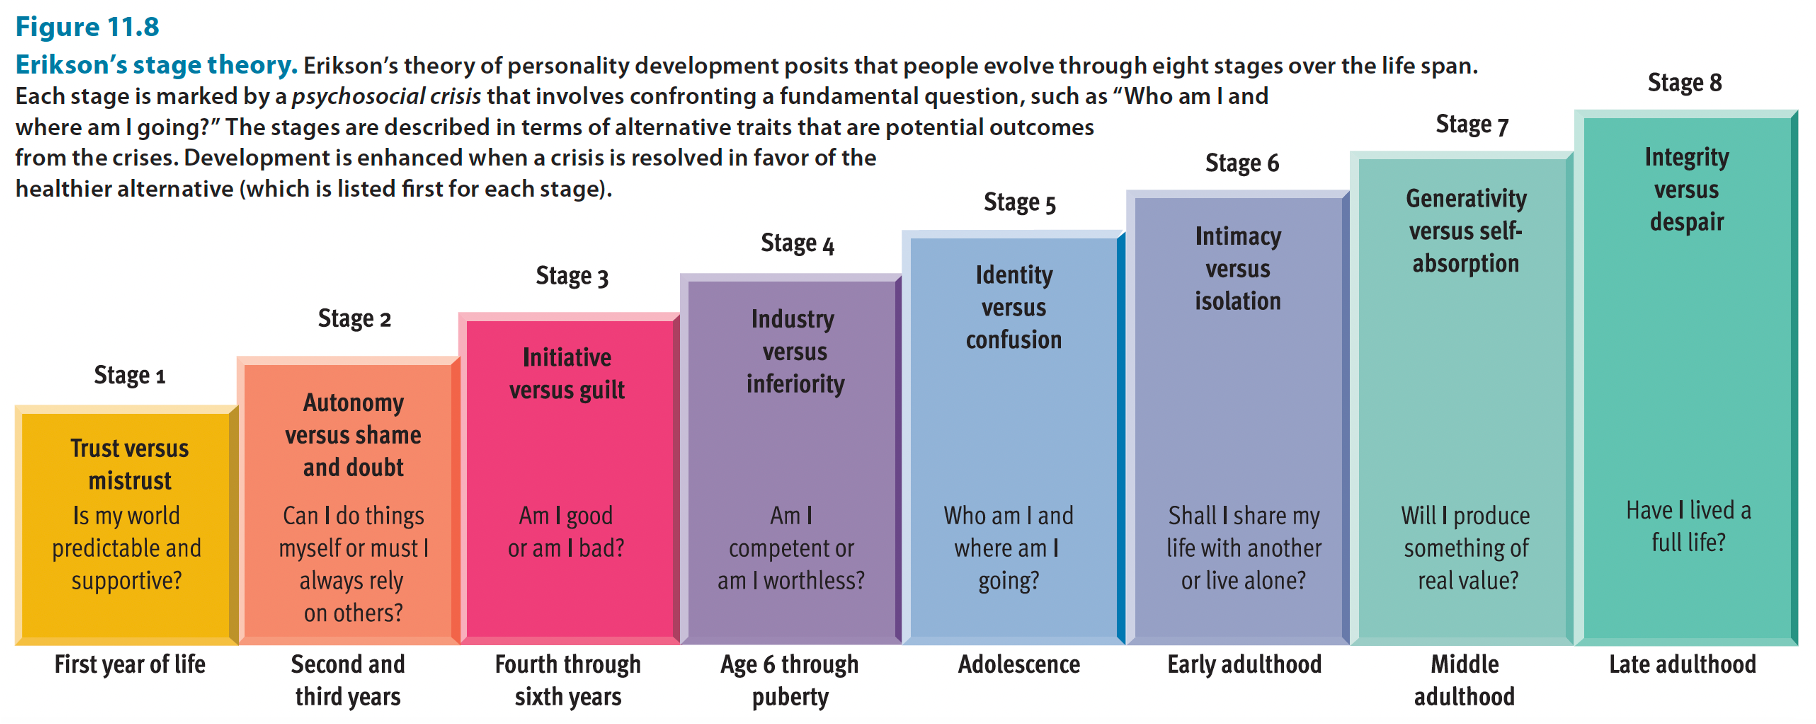
\includegraphics{stages.png}
\end{frame}

\begin{frame}{Marcia's identity statuses}
\phantomsection\label{marcias-identity-statuses}
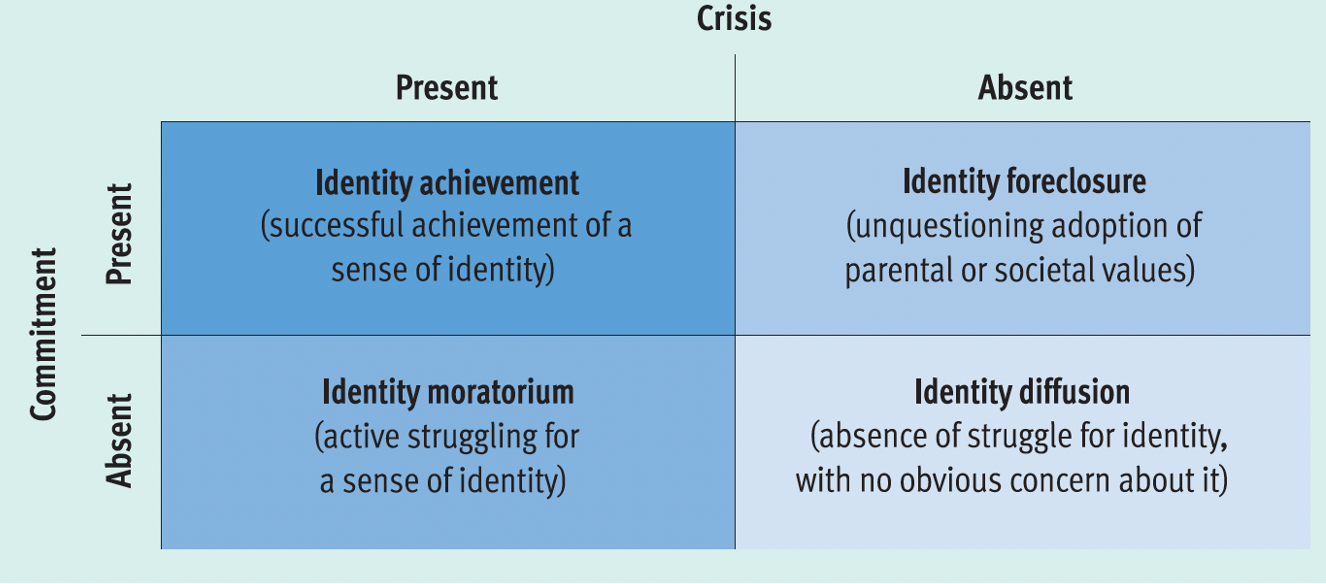
\includegraphics{marcia.png} Identity achievement is associated with
higher self-esteem, conscientiousness, security, achievement motivation,
and capacity for intimacy (Kroger, 2003).
\end{frame}

\section{Have you been in a condition that people don't believe that you
are a New
Zealander?}\label{have-you-been-in-a-condition-that-people-dont-believe-that-you-are-a-new-zealander}

\begin{frame}{Identity denial}
\phantomsection\label{identity-denial}
\begin{itemize}
\tightlist
\item
  Where are you \emph{really} from?: Asian Americans and identity denial
  (Cheryan \& Monin, 2005)
\item
  Leads to poor psychological health and wellbeing, such as depressive
  symptoms and stress (Albuja et al., 2018)
\end{itemize}
\end{frame}

\begin{frame}{Do you think we have an identity problem?}
\phantomsection\label{do-you-think-we-have-an-identity-problem}
\end{frame}

\begin{frame}{What to do?}
\phantomsection\label{what-to-do}
\begin{itemize}[<+->]
\tightlist
\item
  Individually: coping, awareness, standing up, promoting positive
  intergroup contact, building bridges
\item
  As a group: nurture a strong supportive social network but remember
  that this should not be exclusive!
\end{itemize}
\end{frame}

\begin{frame}{The importance of social support}
\phantomsection\label{the-importance-of-social-support}
\begin{itemize}[<+->]
\tightlist
\item
  Whoever desires an increase in his sustenance and age, should keep
  good relations with kith and kin. Muslim
\item
  Broad. But comes from family, relatives, friends and peers.
\item
  Social support domains: emotional, instrumental, informational, and
  physical affection. These buffer individuals from stressors.
\item
  Offering/giving social support is more beneficial than receiving it:
  reduces distress, and improves physical as well as mental health.
\item
  In married couple mortality was significantly reduced for those who
  reported providing instrumental support to friends, relatives,
  neighbours, and spouses. (Utz, 2011)
\end{itemize}
\end{frame}

\begin{frame}{The importance of family/parenting}
\phantomsection\label{the-importance-of-familyparenting}
\begin{itemize}[<+->]
\tightlist
\item
  Married couples have high wellbeing (emotional and psych) and physical
\item
  Reported being more happy
\item
  Significantly low levels of depression
\item
  Children that grow up in a married two parent family are less likely
  to experience emotional-behavioural problems (Brown, 2004)
\item
  They are less likely to drop out of the school, use drugs, give birth
  as teenagers, or experience child abuse (Flewelling et el., 1990)
\item
  More educated and better educational outcomes (Haurin, 1992).
\end{itemize}
\end{frame}

\begin{frame}{Muslims with the strongest ties to their community as
measured by service attendance and prayer are buffered most from
anti-Muslim prejudice.}
\phantomsection\label{muslims-with-the-strongest-ties-to-their-community-as-measured-by-service-attendance-and-prayer-are-buffered-most-from-anti-muslim-prejudice.}
\end{frame}

\begin{frame}{Muslims experience greater challenges to employment and
health than matched members of other religious groups.}
\phantomsection\label{muslims-experience-greater-challenges-to-employment-and-health-than-matched-members-of-other-religious-groups.}
Subjective well-being, the meaning of life, and psychological distress
are similar among Muslims and matched members of religious groups from
the buffering of religious community-making.
\end{frame}

\begin{frame}{Muslim Diversity Study}
\phantomsection\label{muslim-diversity-study}
\begin{figure}

\begin{minipage}{\linewidth}
\begin{center}

\includegraphics[width=0.5\textwidth,height=\textheight]{mds.png}
\end{center}
\end{minipage}%
\newline
\begin{minipage}{\linewidth}

\includegraphics{sponsors.png}\end{minipage}%

\end{figure}%
\end{frame}

\begin{frame}{Our research into the perception of Muslim community
(2016-present)}
\phantomsection\label{our-research-into-the-perception-of-muslim-community-2016-present}
\begin{itemize}[<+->]
\tightlist
\item
  Perception of Muslim in New Zealand
\item
  Who is a true New Zealander?
\item
  Change in attitudes post March 15 attacks
\end{itemize}
\end{frame}

\begin{frame}{But\ldots. it does not raise the Muslim voice}
\phantomsection\label{but.-it-does-not-raise-the-muslim-voice}
\end{frame}

\begin{frame}{Muslim Diversity Study covers}
\phantomsection\label{muslim-diversity-study-covers}
\begin{itemize}[<+->]
\tightlist
\item
  Muslims self-perception, perception of discrimination, diversity,
  flourishing, wellbeing, meaning-making, resilience, and health
  outcomes.
\item
  More importantly, effects of religion and religious support.
\end{itemize}
\end{frame}

\begin{frame}{More importantly, effects of religion and religious
support.}
\phantomsection\label{more-importantly-effects-of-religion-and-religious-support.}
\end{frame}

\begin{frame}{Increase Muslim community representation}
\phantomsection\label{increase-muslim-community-representation}
\end{frame}

\begin{frame}{Increase research opportunities for the Muslim community}
\phantomsection\label{increase-research-opportunities-for-the-muslim-community}
\end{frame}

\begin{frame}{Share findings back with the community members,
leadership, and government.}
\phantomsection\label{share-findings-back-with-the-community-members-leadership-and-government.}
\end{frame}

\begin{frame}{Are my responses confidential?}
\phantomsection\label{are-my-responses-confidential}
Can they be linked back to me?
\end{frame}

\begin{frame}{How does it help Muslim community in the long run?}
\phantomsection\label{how-does-it-help-muslim-community-in-the-long-run}
\end{frame}

\begin{frame}{How can you participate?}
\phantomsection\label{how-can-you-participate}
blah blah blah
\end{frame}

\begin{frame}{MDS Team}
\phantomsection\label{mds-team}
\begin{columns}[T]
\begin{column}{0.4\textwidth}
contents\ldots{}
\end{column}

\begin{column}{0.6\textwidth}
contents\ldots{}
\end{column}
\end{columns}
\end{frame}

\begin{frame}{MDS Core Team}
\phantomsection\label{mds-core-team}
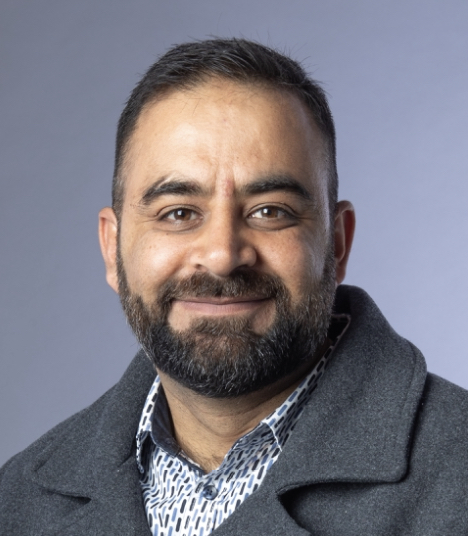
\includegraphics{usman-a.jpeg} 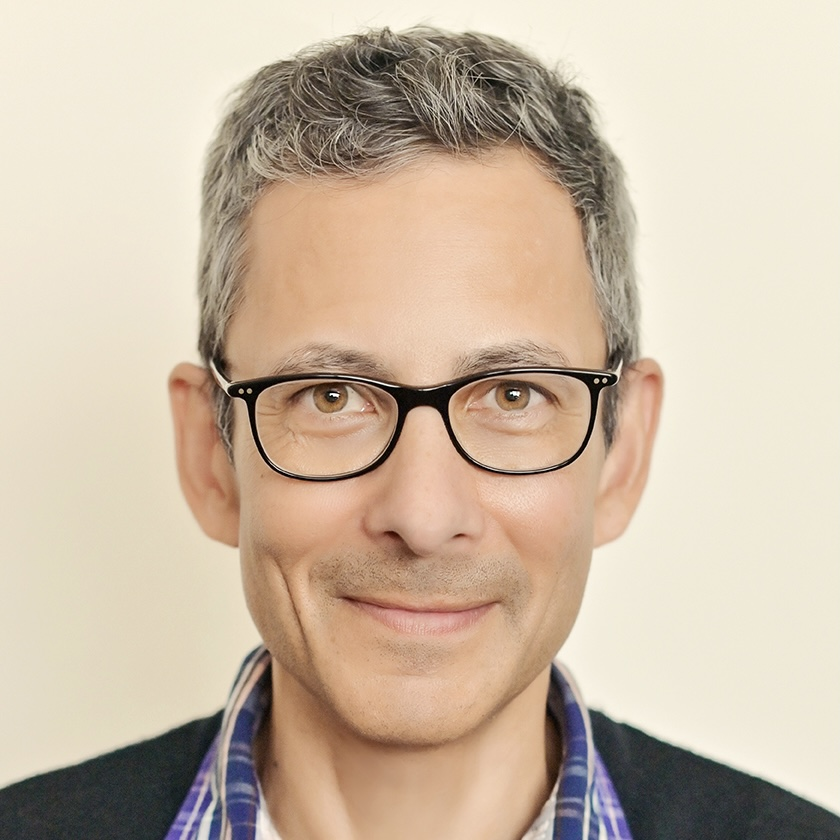
\includegraphics{joe-b.jpg}
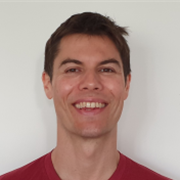
\includegraphics{chris-s.png} 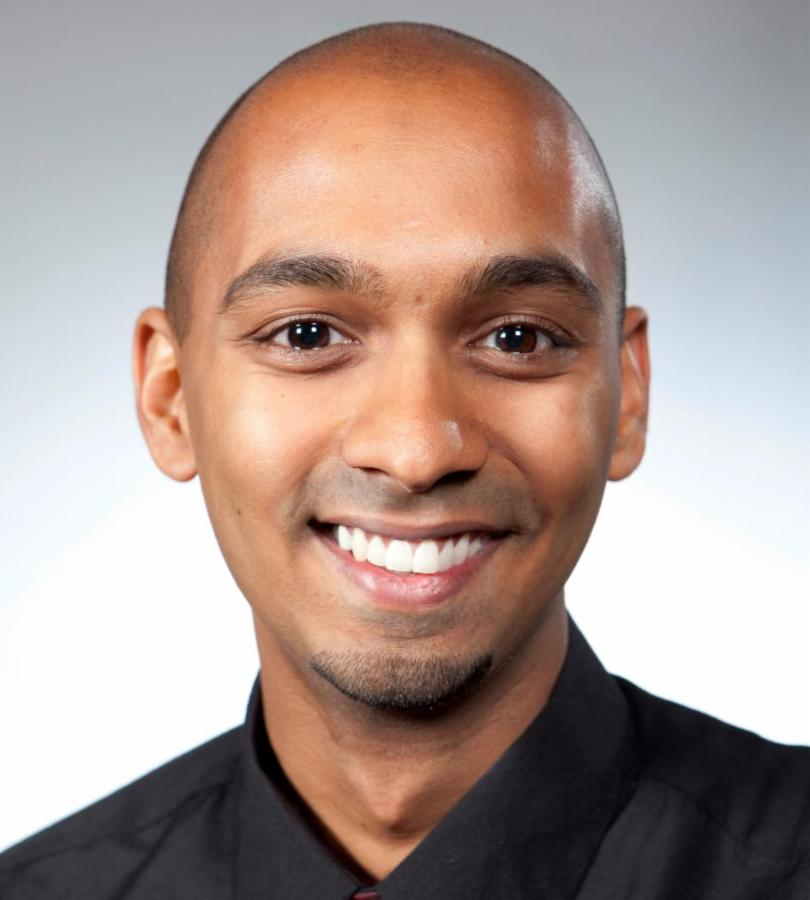
\includegraphics{kumar-y.jpg}
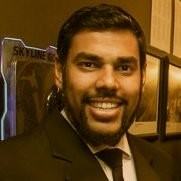
\includegraphics{aarif-r.jpeg}
\end{frame}

\begin{frame}{Team}
\phantomsection\label{team}
\begin{itemize}
\tightlist
\item
  20+ Research Assistants
\item
  Numerous research collaborators
\item
  Muslim Reference Group
\end{itemize}
\end{frame}

\begin{frame}{Thanks to}
\phantomsection\label{thanks-to}
MSA Library Salam Aotearoa Afghan Association of NZ
\end{frame}

\begin{frame}{Special Thanks to MDS Auckland Team}
\phantomsection\label{special-thanks-to-mds-auckland-team}
\end{frame}



\end{document}
